\chapter{Polymorphism: One Interface, Many Forms}

\section{Introduction: Real-Life Hook}

In a classroom:
\begin{itemize}
    \item A student answers questions
    \item A teacher explains lessons
    \item A principal gives instructions
\end{itemize}

All of them can \textbf{speak}, but each speaks in a different way.

This idea —
\begin{center}
\textit{same action, different behavior}
\end{center}

is called \textbf{Polymorphism} in programming.

\section{Concept: What Is Polymorphism?}

\begin{definition}{Polymorphism}
Polymorphism is an OOP concept where \textbf{the same method name behaves differently for different objects}.
\end{definition}

The word comes from Greek:
\begin{itemize}
    \item \textbf{Poly} = many
    \item \textbf{Morph} = forms
\end{itemize}

So, polymorphism means:
\begin{center}
\textit{many forms of the same action}
\end{center}

\section{Why Polymorphism Is Important}

\begin{itemize}
    \item Makes programs flexible
    \item Reduces complex conditional code
    \item Improves code readability
    \item Supports real-life modeling
\end{itemize}

\section{Polymorphism Using Inheritance}

Polymorphism often works together with inheritance.

\begin{verbatim}
class Person:
    def role(self):
        print("I am a person")

class Student(Person):
    def role(self):
        print("I am a student")

class Teacher(Person):
    def role(self):
        print("I am a teacher")
\end{verbatim}

\begin{verbatim}
people = [Student(), Teacher()]

for p in people:
    p.role()
\end{verbatim}

\textbf{Output:}
\begin{verbatim}
I am a student
I am a teacher
\end{verbatim}

Same method name \texttt{role()}, different behavior.

\section{Method Overriding}

\begin{definition}{Method Overriding}
Method overriding occurs when a child class provides its own implementation of a parent class method.
\end{definition}

\begin{verbatim}
class Animal:
    def sound(self):
        print("Animal makes a sound")

class Dog(Animal):
    def sound(self):
        print("Dog barks")
\end{verbatim}

\begin{verbatim}
a = Animal()
d = Dog()

a.sound()
d.sound()
\end{verbatim}

\section{Polymorphism Without Inheritance (Duck Typing)}

In Python, objects do not need to share a parent class.

\begin{verbatim}
class Pen:
    def write(self):
        print("Writing with pen")

class Keyboard:
    def write(self):
        print("Typing with keyboard")
\end{verbatim}

\begin{verbatim}
items = [Pen(), Keyboard()]

for item in items:
    item.write()
\end{verbatim}

If it behaves like a duck, Python treats it like a duck.

\section{Mini-Project: Notification System}

\textbf{Goal:} Send messages using different methods.

\begin{verbatim}
class Email:
    def send(self):
        print("Sending email")

class SMS:
    def send(self):
        print("Sending SMS")

class AppNotification:
    def send(self):
        print("Sending app notification")
\end{verbatim}

\begin{verbatim}
notifications = [Email(), SMS(), AppNotification()]

for n in notifications:
    n.send()
\end{verbatim}

Students learn:
\begin{itemize}
    \item Same method name
    \item Different implementations
    \item Cleaner code design
\end{itemize}

\section{Diagram: Polymorphism Concept}

\begin{center}
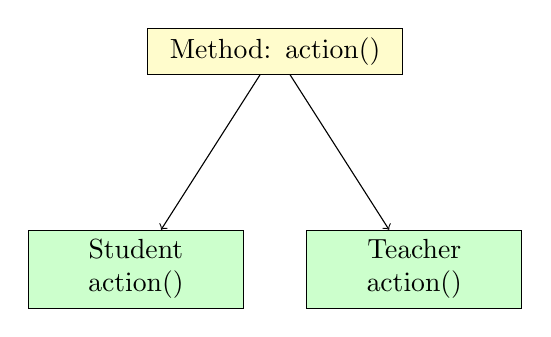
\begin{tikzpicture}[node distance=2.5cm]
\node (base) [draw, rectangle, fill=yellow!20, text width=3cm, align=center] {Method: action()};
\node (c1) [draw, rectangle, fill=green!20, below left of=base, yshift=-1cm, text width=2.5cm, align=center] {Student\\
action()};
\node (c2) [draw, rectangle, fill=green!20, below right of=base, yshift=-1cm, text width=2.5cm, align=center] {Teacher\\
action()};

\draw[->] (base) -- (c1);
\draw[->] (base) -- (c2);
\end{tikzpicture}
\end{center}

\section{Key Concepts}

\begin{itemize}
    \item Polymorphism means many forms
    \item Same method name, different behavior
    \item Achieved using inheritance and overriding
    \item Python supports duck typing
\end{itemize}

\section{Common Beginner Mistakes}

\begin{itemize}
    \item Forgetting to override method correctly
    \item Using different method names
    \item Overusing conditionals instead of polymorphism
\end{itemize}

\section{End-of-Chapter Exercises}

\subsection{Very Short Questions}

\begin{enumerate}
    \item What does polymorphism mean?
    \item Which OOP concept allows method overriding?
    \item What is duck typing?
\end{enumerate}

\subsection{Short Answer Questions}

\begin{enumerate}
    \item Explain polymorphism using a real-life example.
    \item Write a parent class and two child classes demonstrating polymorphism.
    \item Why is polymorphism useful in large programs?
\end{enumerate}

\subsection{Activity-Based Exercises}

\begin{enumerate}
    \item Create a \texttt{Shape} class and override \texttt{area()} in Circle and Rectangle.
    \item Design a \texttt{Payment} system with Cash, Card, and MobilePayment classes.
    \item Rewrite an \texttt{if-else} based program using polymorphism.
\end{enumerate}

\section{Teacher Notes}

\marginnote{
\textbf{Learning Objectives}
\begin{itemize}
    \item Students understand polymorphism clearly
    \item Students apply method overriding
    \item Students write flexible programs
\end{itemize}

\textbf{Teaching Tips}
\begin{itemize}
    \item Demonstrate same method name on different objects
    \item Compare with real-life roles
    \item Emphasize clean code design
\end{itemize}

\textbf{Assessment}
\begin{itemize}
    \item Correct overriding
    \item Proper use of polymorphism
\end{itemize}
}